\chapter[Resultados e Análise dos Resultados]{Resultados e Análise dos Resultados}

\section{Consumo de Combustível}
A tabela \ref{tabela_resultados} apresenta os resultados do experimento com o motor operando somente com gasolina, a duplo combustível com o gaseificador a topo aberto e a topo fechado. 

\begin{table}[h]
	\centering
	\caption{Resultados do experimento. (Fonte: autoria própria)}
	\begin{tabular}{|c|c|c|c|c|c|}
		\hline
		Combustível & Rotação & Tempo & Posição & Pressão & Consumo	\\
		& do Motor & de Injeção & da Borboleta & Coletor & \\
		& (rpm) & (ms) & (graus) & (mmHg) & (L/h)\\
		\hline
		\multirow{12}{4.5cm}{Gasolina}
		& 926 & 0,52 & 14 & 388 & 1,63 x 10\textsuperscript{-1}\\
		& 969 & 0,55 & 14 & 355 & 1,80 x 10\textsuperscript{-1}\\
		& 984 & 0,53 & 14 & 352 & 1,76x 10\textsuperscript{-1}\\
		& 3597 & 0,54 & 24 & 283 & 6,57 x 10\textsuperscript{-1} \\
		& 4007 & 0,44 & 24 & 460 & 5,96 x 10\textsuperscript{-1}\\
		& 4038 & 0,68 & 24 & 470 & 9,28 x 10\textsuperscript{-1}\\
		& 4046 & 0,49 & 24 & 271 & 6,70 x 10\textsuperscript{-1}\\
		& 4056 & 0,66 & 24 & 259 & 9,05 x 10\textsuperscript{-1}\\
		& 4061 & 0,66 & 24 & 450 & 9,06 x 10\textsuperscript{-1}\\
		& 4071 & 0,65 & 24 & 259 & 8,94 x 10\textsuperscript{-1}\\
		& 4107 & 0,68 & 24 & 259 & 9,44 x 10\textsuperscript{-1}\\
		\hline
		\multirow{12}{4.5cm}{Gasolina + syngas (Topo aberto)}
		& 3532 & 0,49 & 24 & 283 & 5,85 x 10\textsuperscript{-1}\\
		& 3579 & 0,48 & 24 & 280 & 5,81 x 10\textsuperscript{-1}\\
		& 3656 & 0,49 & 24 & 280 & 6,06 x 10\textsuperscript{-1}\\
		& 3838 & 0,61 & 24 & 259 & 7,91 x 10\textsuperscript{-1}\\
		& 4009 & 0,68 & 24 & 259 & 9,08 x 10\textsuperscript{-1}\\
		& 4021 & 0,67 & 24 & 262 & 9,11 x 10\textsuperscript{-1}\\
		& 4035 & 0,65 & 24 & 259 & 8,86 x 10\textsuperscript{-1}\\
		& 4038 & 0,64 & 24 & 259 & 8,74 x 10\textsuperscript{-1}\\
		& 4047 & 0,64 & 24 & 259 & 8,75 x 10\textsuperscript{-1}\\
		& 4061 & 0,65 & 24 & 259 & 8,92 x 10\textsuperscript{-1}\\
		& 4162 & 0,68 & 24 & 265 & 9,57 x 10\textsuperscript{-1}\\
		\hline
		\multirow{12}{4.5cm}{Gasolina + syngas (Topo fechado)}
		& 887 & 0,65 & 14 & 409 & 1,95 x 10\textsuperscript{-1}\\
		& 893 & 0,65 & 14 & 466 & 3,68 x 10\textsuperscript{-1}\\
		& 926 & 0,88 & 14 & 388 & 2,75 x 10\textsuperscript{-1}\\
		& 927 & 0,71 & 14 & 415 & 2,22 x 10\textsuperscript{-1}\\
		& 2767 & 0,81 & 22 & 301 & 7,58 x 10\textsuperscript{-1}\\
		& 2794 & 0,50 & 22 & 301 & 4,72 x 10\textsuperscript{-1}\\
		& 2805 & 1,02 & 22 & 298 & 9,67 x 10\textsuperscript{-1}\\
		& 2858 & 0,52 & 22 & 289 & 5,02 x 10\textsuperscript{-1}\\
		& 2868 & 0,68 & 23 & 301 & 6,59 x 10\textsuperscript{-1}\\
		& 2875 & 0,63 & 22 & 289 & 6,12 x 10\textsuperscript{-1}\\
		& 3026 & 0,81 & 23 & 292 & 8,28 x 10\textsuperscript{-1}\\	
		\hline
	\end{tabular}
	\label{tabela_resultados}
\end{table}	

A figura \ref{grafico_consumo} mostra um gráfico representando o consumo do motor com as diferentes configurações de combustível analisadas.

\begin{figure}[!htb]
	\centering
	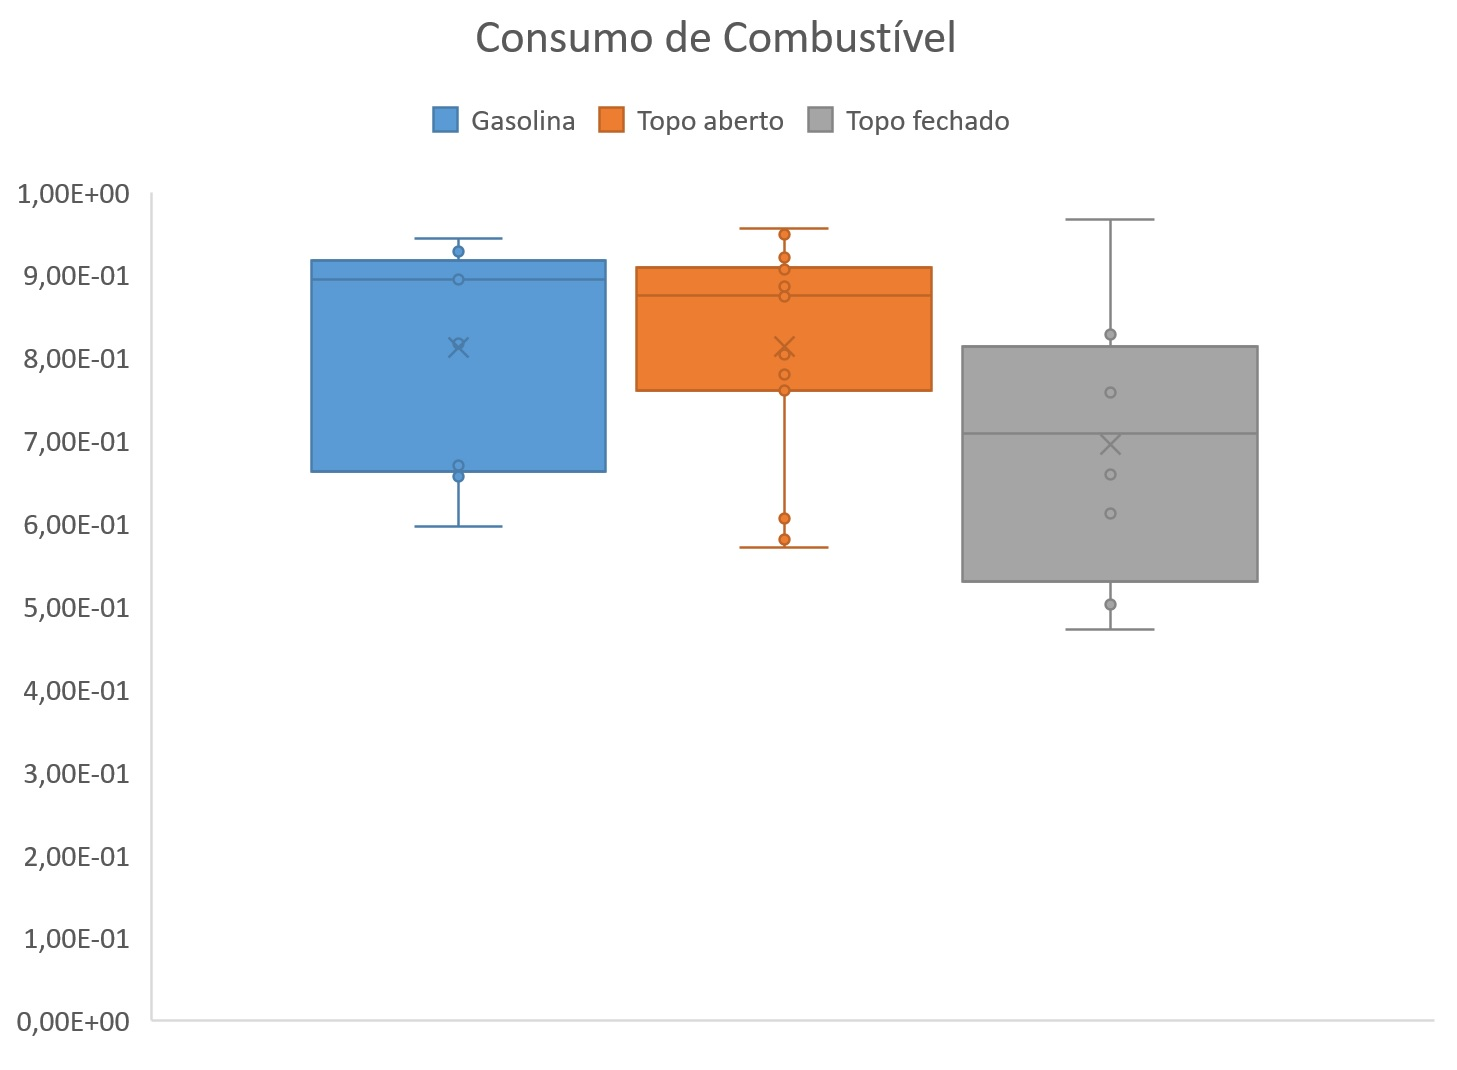
\includegraphics{Figuras/consumo_combustivel}
	\caption{Consumo de Combustível}
	\label{grafico_consumo}
\end{figure}

Trabalhando a duplo combustível com topo aberto, o abatimento no consumo de gasolina  com a adição do gás de síntese foi de 0,13\%. Ao pressurizar o sistema trabalhando com o topo fechado, essa diferença de consumo se mostra mais evidente, chegando a uma redução de 14,4\%.

Esse resultado insatisfatório do gás de síntese no consumo do motor pode ser explicado pela perda de carga na mangueira de entrada de gases, uma vez que esta apresentava diâmetro muito pequeno e, de acordo com a fórmula de Darcy-Weibasch, a perda de carga e o diâmetro da tubulação são inversamente proporcionais, ou seja, quanto menor o diâmetro, maior a perda de carga.

\begin{equation} \label{darcy-weibasch}
 h\textsubscript{f} = f\textsubscript{d}\frac{L}{D}\frac{V^2}{2g}
\end{equation}

Onde f\textsubscript{D} é o coeficiente de atrito, L é o comprimento, D é o diâmetro, $\rho$ é massa específica e V é a velocidade.

\section{Geração de Energia}

A tabela \ref{tabela_resultados_2} mostra o resultado dos cálculos realizados com os dados coletados durante o experimento. Considerou-se os cálculos com 200 gramas de biomassa a topo fechado consumida durante o tempo \textit{t} ocupando metade da altura do reator.

\begin{table}[h]
	\centering
	\caption{Cálculos realizados com os dados coletados. (Fonte: autoria própria)}
	\begin{tabular}{|l|c|c|c|}
		\hline
		Variável & Símbolo & Valor & Equação \\
		\hline
		
		Área da seção transversal & A\textsubscript{g} & 0,01227m\textsuperscript{2} & - \\
		
		Altura da coluna de biomassa & h$_b$ & 0,25m & -\\
		
		Massa específica aparente & $\rho$\textsubscript{ap} & 65,2 kg/m\textsuperscript{3} & - \\
		
		Tempo de comsumo da biomassa & t & 9min ou 0,15h & -\\
		
		Vazão mássica de biomassa & $\dot{m}$\textsubscript{biomassa} & 1,33 kg/h & Eq. \ref{vazao_biomassa_PCI}\\
		
		Taxa específica de processamento do reator & $\psi$ & 105 kg/m\textsuperscript{2}h & Eq. \ref{taxa_reator}\\
		
		\rowcolor{lightgray} Poder Calorífico do syngas & PCI\textsubscript{syngas} & 5,07 MJ/Nm\textsuperscript{3} & Eq. \ref{PCI_Tiangco}\\
		
		Vazão volumétrica do bagaço & $\dot{Q}$\textsubscript{bagaço} & 0,024m\textsuperscript{3}/h & Eq. \ref{qdot_bagaco}\\
		
		Vazão volumétrica do ar & $\dot{Q}$\textsubscript{ar} & 1,2Nm\textsuperscript{3}/h & -\\
		
		Vazão volumétrica do gás de síntese & $\dot{Q}$\textsubscript{syngas} & 1,224Nm\textsuperscript{3}/h & Eq. \ref{balanco_massa}\\
		
		\rowcolor{lightgray} Potência térmica & P\textsubscript{t} & 1.724 W & Eq. \ref{potencia_termica}\\
		
		\hline
\end{tabular}
\label{tabela_resultados_2}
\end{table}	

Segundo \cite{brunetti2012}, a máxima eficiência térmica de um motor de combustão interna é a eficiência do ciclo de Carnot para as condições máximas e mínimas de temperatura neste tipo de motor, resultando numa eficiência máxima de 57,2\%.
Com base nas equações \ref{potencia_eixo} e \ref{potencia_eletrica}, traça-se um gráfico com as potências de eixo e potência elétrica que podem ser geradas em função da eficiência e da potência térmica do syngas, assumindo eficiências entre 10\% e 60\% para $\eta$\textsubscript{motor} e 90\% para $\eta$\textsubscript{g}.

\begin{figure}[!htb]
	\centering
	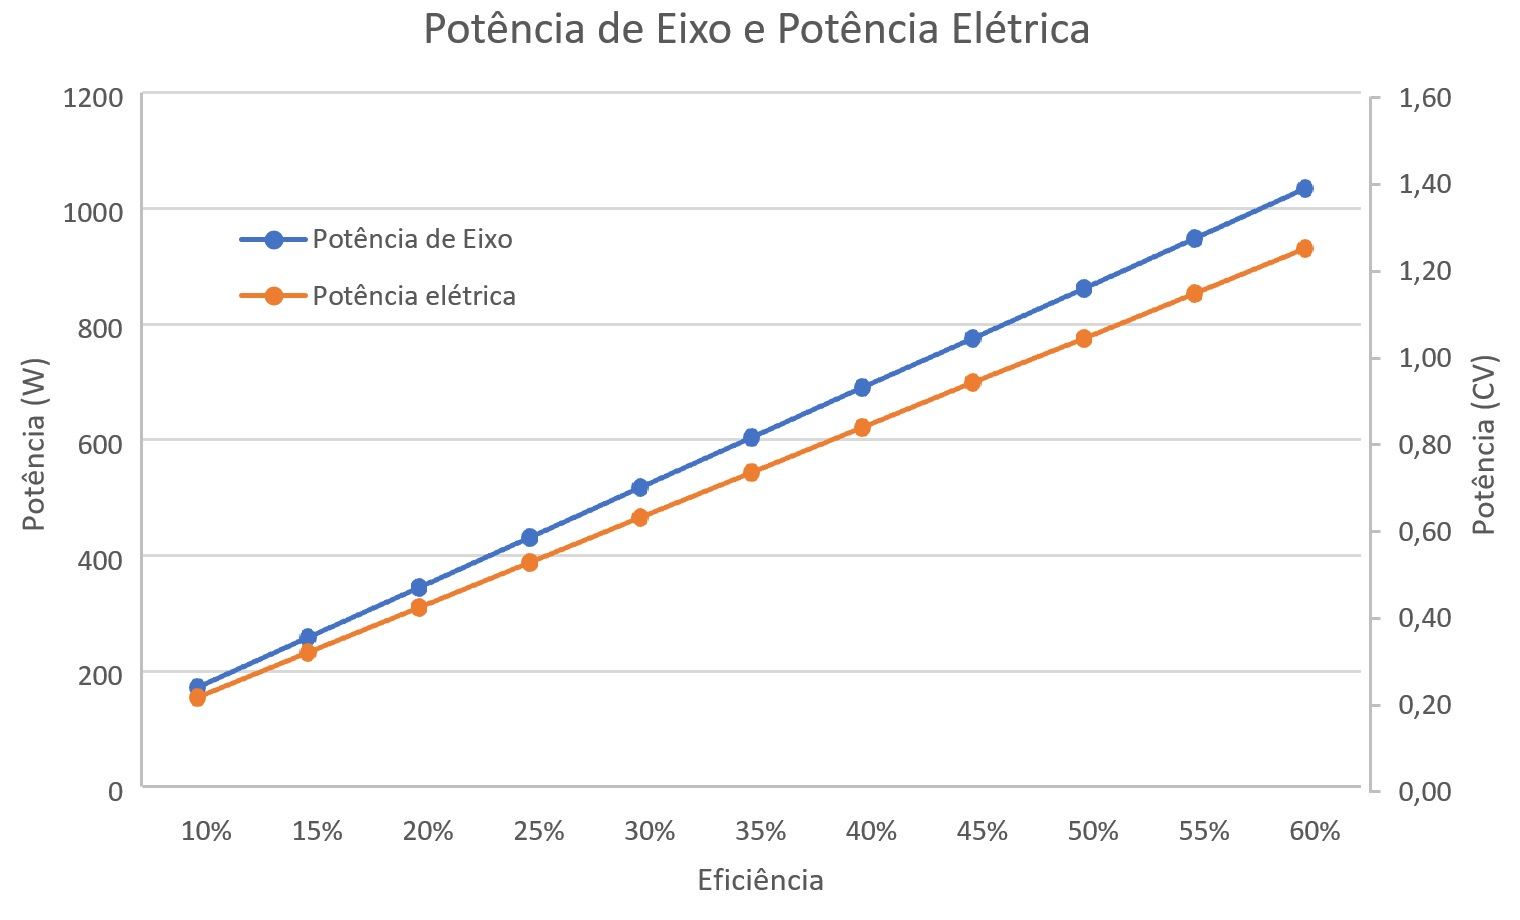
\includegraphics[width=14cm]{Figuras/grafico_potencia_eficiencia_2}
	\caption{Gráfico das potências de eixo e elétrica.}
	\label{grafico_potencia_eficiencia}
\end{figure}



Portanto, um motor a combustão genérico com eficiência de até 57\%, trabalhando com gás de síntese do bagaço de cana com uma potência térmica de 1.724W, sem condiserar as demais perdas do sistema, seria capaz de movimentar uma moenda de cana de até 1,3cv acoplada ao seu eixo. Acoplando um gerador, o conjunto moto-gerador supriria um motor elétrico de até 1,2cv.

Na tabela \ref{tabela_moendas}, seguem as especificações de diferentes modelos de moenda da marca Maqtron, de acordo com seu catálogo.

\begin{table}[h]
	\centering
	\caption{Tabela de moendas de cana marca Maqtron \cite{catalogo2016}}
	\begin{tabular}{|c|c|c|}
	\hline
	\rowcolor{lightgray}\textbf{Modelo Moenda} & \textbf{Motor elétrico indicado} & \textbf{Motor estacionário indicado} \\
	\rowcolor{lightgray} & \textbf{[CV]} & \textbf{[CV]} \\
	\hline
	Cana Express Hobby & 1/2 & - \\
	Cana Shop 60 & 1/2 & - \\
	Cana Shop 140 & 1 & - \\
	Cana Shop 200 & 2 & - \\
	Cana Shop Estacionária & - & 3,5 - 5,0 \\
	B-721 Turbo & 1,5 - 2,0 & 3,5 \\
	B-722 Turbo & 1,2 - 2,0 & 3,5 \\
	M-700 & 1 & - \\
	B-728 & 1/2 & - \\
	B-723 & 1/2 - 1,0 & - \\
	B-730 & 5 a 7,5 & 8 a 12 \\
	\hline
	\end{tabular}
	\label{tabela_moendas}
\end{table}	

Para esses modelos de moenda, seria necessário um motor a combustão com potência de eixo mínima de 3,5cv. Portanto, qualquer motor a combustão necessitaria trabalhar a duplo combustível para suprir a demanda de potência de tais moendas, uma vez que a energia do gás de síntese sozinho não é capaz de fornecer potência suficiente.

Um gerador acoplado ao motor seria capaz de suprir a demanda de potência de motores elétricos de sete das onze moendas da tabela \ref{tabela_moendas}, as demais necessitariam também que o motor trabalhasse a duplo combustível. Para moendas pequenas que demandam potência do motor elétrico de 1/2 cv, seria necessário um moto-gerador com eficiência mínima de 23,5\%.

A partir dos dados coletados, pôde-se calcular a potência de eixo que pode ser fornecida pelo motor a combustão utilizado neste experimento. Considerou-se para os cáluclos os dados de gasolina quando o motor estava operando a duplo combustível com topo fechado. Uma vez que não há dados suficientes para avaliar a potência que pode ser gerada com o gás de síntese que de fato entrou no motor, considerou-se, para o syngas, os resultados teóricos calculados e expostos na tabela \ref{tabela_resultados}. Na tabela \ref{tabela_potencia_motor_fiat}, vê-se o resultado da potência de eixo do motor com tais dados.

\begin{table}[h]
	\centering
	\caption{Resultados do motor utilizado}
	\begin{tabular}{|l|c|}
		\hline
		\rowcolor{lightgray} Variável & Valor \\
		\hline
		Consumo de gasolina médio & 0,696 L/h \\
		Massa específica gasolina & 720 kg/m$^3$ \\
		Vazão mássica de gasolina & 0,501 kg/h \\
		Poder Calorífico Inferior gasolina & 43 MJ/kg \\
		Potência térmica gasolina & 5,985 kW ou 8 cv\\
		Potência térmica syngas & 1,724 kW ou 2,3 cv \\
		Eficiência máxima de um MCI & 57\% \\
		 Potência de eixo gasolina & 3,41 kW ou 4,6 cv \\
		 Potência de eixo syngas & 982,68W ou 1,3 cv \\
		 Potência de eixo total & 4,39kW ou 6 cv \\
		\hline
	\end{tabular}
	\label{tabela_potencia_motor_fiat}
\end{table}	


Trabalhando a duplo combustível, somente a parcela de gasolina já é capaz de fornecer potência necessária para movimentar as moendas de cana da tabela \ref{tabela_moendas}, exceto a de modelo B-730. 
Ao acoplar um gerador a esse motor, a potência fornecida ao motor elétrico seria de 5,4 cv, considerando os dois combustíveis, o que também supriria a demanda das moendas da tabela.

\section{Análise Financeira}

A análise financeira será realizada através de uma análise teórica em que um gerador de energia elétrica com eficiência de 90\% seria acoplado ao motor utilizado no experimento e injetaria energia elétrica na rede de distribuição.

Fez-se levantamento de dados de uma pastelaria situada no setor central da cidade do Gama, DF. Foi anotado quais eram os equipamentos elétricos utilizados no estabelecimento e suas respectivas especificações técnicas, bem como o tempo que ficam ligados, esses resultados encontram-se na tabela \ref{dados_pastelaria}. A pastelaria funciona das 8h às 17hs e gera aproximadamente 15kg de bagaço por dia, a moenda utilizada no estabelecimento é o modelo CanaShop 140

\begin{table}[h]
	\centering
	\caption{Dados dos equipamentos elétricos da pastelaria.}
	\begin{tabular}{|c|c|c|c|c|}
		\hline
		\rowcolor{lightgray} Quantidade & Equipamento & Potência (W) & Horas (h) & Consumo mensal \\
		\rowcolor{lightgray}& & & & (kWh/mês) \\
		\hline
		1 & Moenda de Cana & 735 W & 9 & 158,8 \\
		1 & Fritadeira elétrica & 2500 & 9 & 540 \\
		2 & Freezer & 500 & 9 & 216 \\
		1 & Geladeira & 300 & 9 & 64,8\\
		1 & Cilindro de massa & 735 & 9 & 158,8\\
		1 & Estufa para salgados & 200 & 9 & 43,2\\
		1 & Microondas & 1000 & 2 & 48 \\
		\hline
		\rowcolor{lightgray}\multicolumn{4}{|r|}{\textbf{Consumo mensal total}} & \textbf{1.230 kWh/mês} \\
		\hline
	\end{tabular}
	\label{dados_pastelaria}
\end{table}	

Segundo site da ANP, o preço da gasolina para o estado do Distrito Federal no mês de junho é de R\$ 4,40 \cite{anp}. Segundo a CEB, a tarifa de energia para o grupo A referente aos consumidores comerciais em bandeiras verde e vermelha são, R\$ 0,53/kWh e R\$ 0,75/kWh, respectivamente \cite{ceb}. Portanto, os custos mensais da pastelaria com energia elétrica antes e após a inserção do sistema de gaseificação proposto podem ser vistos na tabela \ref{custos_finais}.

A energia elétrica mensal produzida pelo sistema de gaseificação proposto é de 854kWh/mês, segundo cálculo resultante da equação abaixo.

\begin{center}
	Energia produzida = Potência de eixo total * $\eta$\textsubscript{g} * horas mensais
	
	Energia produzida = 4,39kW * 0,9 * 216h/mês
	
	Energia produzida = 854kWh/mês
	
\end{center}



\begin{table}[h]
	\centering
	\caption{Custos de energia com e sem o sistema de gaseificação.}
	\begin{tabular}{|c|c|c|c|}
		\hline
		Consumo de gasolina mensal & Preço da gasolina & Custo mensal &\\
		& & da gasolina & \\
		150L/mês & R\$ 4,40/L & R\$ 660,00 &\\
		\hline
		\rowcolor{gray} \multicolumn{4}{|c|}{} \\
		\hline
		Energia elétrica consumida & \multicolumn{2}{c|}{Bandeira Verde}  & Custo Mensal\\
		\cline{2-3}
		sem sistema de gaseificação &  Tarifa & Custo Mensal & Total\\
		\multirow{4}{*}{1230 kWh/mês} & R\$ 0,53/kWh &  R\$ 651,90 & \cellcolor{lightgray} R\$ 651,90 \\
		\cline{2-4}
		& \multicolumn{2}{c|}{Bandeira Vermelha}  & Custo Mensal\\
		\cline{2-3}
		& Tarifa  & Custo Mensal & Total\\
		& R\$ 0,75/kWh &  R\$ 922,50 & \cellcolor{lightgray} R\$ 922,50 \\
		\hline
		\rowcolor{gray} \multicolumn{4}{|c|}{} \\
		\hline
		Energia elétrica consumida & \multicolumn{2}{c|}{Bandeira Verde}  & Custo Mensal \\
		\cline{2-3}
		com sistema de gaseificação & Tarifa  & Custo Mensal & Total\\
		\multirow{4}{*}{376 kWh/mês} & R\$ 0,53/kWh & R\$ 199,28 & \cellcolor{lightgray} R\$ 859,28\\
		\cline{2-4}
		& \multicolumn{2}{c|}{Bandeira Vermelha}  & Custo Mensal\\
		\cline{2-3}
		& Tarifa  & Custo Mensal &  Total \\
		& R\$ 0,75/kWh & R\$ 282,00 & \cellcolor{lightgray}R\$ 942,00\\
		\hline
		\rowcolor{gray} \multicolumn{4}{|c|}{} \\
		\hline
	\end{tabular}
	\label{custos_finais}
\end{table}	

O custo mensal total de energia elétrica consumida com sistema de gaseificação é a soma do custo da energia elétrica mais o custo mensal da gasolina utilizada no motor a combustão.

Ao introduzir o sistema de gaseificação, o custo mensal aumenta 24,1\% em bandeira verde e 2,97\% em bandeira vermelha. Este aumento se deve ao alto preço por litro da gasolina, uma vez que esta fonte energética está sendo responsável por 76,8\% do custo total mensal em bandeira verde e 70\% em bandeira vermelha.

Para que o sistema de gaseificação se torne viável economicamente, o preço por litro da gasolina deve ser, no máximo, R\$ 3/L em bandeira verde e R\$ 4,27/L em bandeira vermelha. Mantendo-se o atual preço da gasolina, a viabilidade econômica também seria possível em um sistema em que a inserção do gás de síntese reduzisse em, pelo menos, 64,5\% o consumo de gasolina no motor, passando de 0,814L/h para 0,289L/h. Neste caso, o custo mensal em bandeira verde não se alteraria, e haveria uma redução de 12,36\% em bandeira vermelha, como pode ser visto na tabela \ref{custos_reducao_gasolina}. Em um cenário em que o motor trabalhasse apenas com o gás de síntese, a redução na conta de energia elétrica da pastelaria seria de 15,5\%.

\begin{table}[h]
	\centering
	\caption{Custos de energia com redução no consumo de gasolina.}
	\begin{tabular}{|c|c|c|c|}
		\hline
		Consumo de gasolina mensal & Preço da gasolina & Custo mensal &\\
		& & da gasolina & \\
		62,4L/mês & R\$ 4,40/L & R\$ 274,67 &\\
		\hline
		\rowcolor{gray} \multicolumn{4}{|c|}{} \\
		\hline
		Energia elétrica consumida & \multicolumn{2}{c|}{Bandeira Verde} & Custo Mensal\\
		\cline{2-3}
		sem sistema de gaseificação & Tarifa & Custo Mensal & Total\\
		\multirow{4}{*}{1230 kWh/mês} & R\$ 0,53/kWh &  R\$ 651,90 & \cellcolor{lightgray} R\$ 651,90 \\
		\cline{2-4}
		& \multicolumn{2}{c|}{Bandeira Vermelha} & Custo Mensal\\
		\cline{2-3}
		& Tarifa  & Custo Mensal & Total\\
		& R\$ 0,75/kWh &  R\$ 922,50 & \cellcolor{lightgray} R\$ 922,50 \\
		\hline
		\rowcolor{gray} \multicolumn{4}{c}{} \\
		\hline
		Energia elétrica consumida & \multicolumn{2}{c|}{Bandeira Verde}  & Custo Mensal \\
		\cline{2-3}
		com sistema de gaseificação & Tarifa  & Custo Mensal & Total\\
		\multirow{4}{*}{712 kWh/mês} & R\$ 0,53/kWh & R\$ 377,22 & \cellcolor{lightgray} R\$ 651,89\\
		\cline{2-4}
		& \multicolumn{2}{c|}{Bandeira Vermelha} & Custo Mensal\\
		\cline{2-3}
		& Tarifa  & Custo Mensal &  Total \\
		& R\$ 0,75/kWh & R\$ 533,804 & \cellcolor{lightgray}R\$ 808,5\\
		\hline
		\rowcolor{gray} \multicolumn{4}{|c|}{} \\
		\hline
	\end{tabular}
	\label{custos_reducao_gasolina}
\end{table}	

Para um usuário que não tenha acesso à rede de distribuição de energia e deseje acoplar ao sistema de gaseificação apenas a fritadeira elétrica, a moenda de cana e o cilindro de massa, o sistema seria viável economicamente, tendo em vista que houve redução no consumo de gasolina e, portanto, também haverá redução de 14,7\% no custo mensal.

